%
%  Getting Started with JavaGP
%
%  Created by Felipe Meneguzzi on 2010-10-31.
%  Copyright (c) 2010 __MyCompanyName__. All rights reserved.
%
\documentclass[]{article}

% Use utf-8 encoding for foreign characters
\usepackage[utf8]{inputenc}

% Setup for fullpage use
\usepackage{fullpage}
\usepackage{hyperref}

% Uncomment some of the following if you use the features
%
% Running Headers and footers
%\usepackage{fancyhdr}

% Multipart figures
%\usepackage{subfigure}

% More symbols
%\usepackage{amsmath}
%\usepackage{amssymb}
%\usepackage{latexsym}

% Surround parts of graphics with box
\usepackage{boxedminipage}

% Package for including code in the document
\usepackage{listings}

% If you want to generate a toc for each chapter (use with book)
\usepackage{minitoc}

% This is now the recommended way for checking for PDFLaTeX:
\usepackage{ifpdf}

%\newif\ifpdf
%\ifx\pdfoutput\undefined
%\pdffalse % we are not running PDFLaTeX
%\else
%\pdfoutput=1 % we are running PDFLaTeX
%\pdftrue
%\fi

\ifpdf
\usepackage[pdftex]{graphicx}
\else
\usepackage{graphicx}
\fi
\title{Getting Started with \textsc{JavaGP}}
\author{Felipe Meneguzzi}

\date{2010-10-31}

\newcommand\exempli{\emph{e.g.}}
\newcommand\idest{\emph{i.e.}}
\newcommand\javagp{\href{http://javagp.sf.net}{\textsc{JavaGP}}}

\begin{document}

\ifpdf
\DeclareGraphicsExtensions{.pdf, .jpg, .tif}
\else
\DeclareGraphicsExtensions{.eps, .jpg}
\fi

\maketitle

% \begin{abstract}
% \end{abstract}

\section{Graphplan}

Graphplan is a planning algorithm based on the construction of and search in a graph \cite{Blum1997}. 
It is considered a breakthrough in terms of efficiency regarding previous approaches to planning \cite{Weld1999, Hoffmann2001}, and has been refined into a series of other, more powerful planners, such as IPP\footnote{Interference Progression Planner} \cite{Koehler1997} and STAN\footnote{State Analysis} \cite{Long1999}, whose efficiency has been empirically verified in several planning algorithm competitions \cite{Long2000,Ghallab2002}.

\begin{figure}[ht]
	\centering
	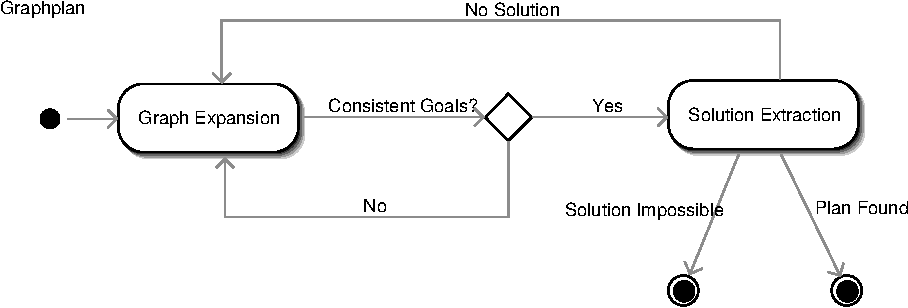
\includegraphics[width=.8\textwidth]{graphplan.pdf}
	\caption{Overview of the Graphplan algorithm.}
	\label{fig:graphplan}
\end{figure}

Planning in Graphplan is based on the concept of a \emph{planning graph}, which is a data structure in which information regarding the planning problem is stored in a directed and levelled graph in such a way that the search for a solution can be optimised. 
The planning graph is not a state-space graph in which a plan is a path through the graph. 
Instead, a plan in the planning graph is essentially a flow in the network flow sense, which is composed of more than one path in a directed graph with the added constraint that paths must not include mutually exclusive nodes in the same graph level.

The planning graph consists of alternating levels of instantiated operators and propositions representing temporally ordered actions and the world-states that occur between the execution of these actions. 
Proposition levels contain nodes labelled with literals, and are connected to the actions in the subsequent action level through precondition arcs. 
Action nodes are labelled with operators and are connected to the nodes in the subsequent proposition nodes by effect arcs. 
Every proposition level denotes literals that are possibly true at a given time step, so the first proposition level represents the literals that are possibly true before plan execution (\exempli time step 1), the next proposition level represents the literals that are possibly true at the next time step (\exempli time step 2) and so forth. 
Action levels denote operators that can be executed at a given moment in time in such a way that the first action level represents the operators that may be executed at time step 1 and so forth. 
The graph contains mutual exclusion relations (\emph{mutex}) between nodes in the same graph level, denoting that two nodes connected by a \emph{mutex} arc cannot be simultaneously present in the same graph level for any solution. 
These mutual exclusion relations play a key role in the efficiency of the algorithm, as the search for a solution can completely ignore any flows that include mutually exclusive nodes in a given level.

Construction of this graph is efficient, having polynomial complexity for both graph size and construction time regarding problem size \cite{Blum1997}. This graph is then used by the planner in the search for a solution to the planning problem using data regarding the relations between operators and states to speed up the search. The basic Graphplan algorithm (\idest without the optimisations proposed by other researchers) is divided into two distinct phases: graph expansion and solution extraction. The algorithm alternates execution of graph expansion and solution extraction until a solution is found or it is proven that no solution exists, as illustrated in Figure~\ref{fig:graphplan}.

\section{Installation and Configuration}
\label{sec:installation}

\begin{enumerate}
\item Java JDK $\geq$ 5.0 is required (\url{http://java.sun.com});
\item Download \javagp from \url{http://javagp.sf.net};
\item Decompress the binary distribution file \texttt{javagp-bin-X.Y.Z.zip}, which creates a folder \texttt{javagp-bin-X.Y.Z}
\item Open a terminal window and go to the uncompressed folder \texttt{cd /path/to/javagp-bin-X.Y.Z}
\item You can now execute \javagp by running \texttt{java -jar javagp.jar}
  % As you can see, \Jason runs as a plugin of
  % \htlink{jEdit}{http://www.jedit.org/} (a text editor developed in
  % Java). This is useful because, although in \Jason agents are
  % programmed in a variant of AgentSpeak, in most cases you'll need to
  % do some Java programming (e.g., if you want to create an environment
  % where the agents are situated).
\item In some cases, it might be necessary to configure the \texttt{PATH} of your system to locate the java executable.
\end{enumerate}

\section{Command Line Interface}
\label{sec:interface}

\textsc{JavaGP} is a command line Java implementation of Graphplan, which takes as input a file describing the \emph{domain} as well as a file describing the \emph{problem}. 
The domain comprises the set of operators available for planning, while the problem describes the initial and goal states. 
A basic invocation of \javagp, then contains references to the domain and the problem (in any order), \exempli \texttt{java -jar javagp.jar -p <problem file> -d <domain file>}. 
Syntax of the domain and problem files is described in Section~\ref{sec:syntax}.
Besides these basic parameters, \javagp can also take the following two parameters:
\begin{itemize}
	\item \texttt{-maxlevels <n>} --- limits the number of graph levels to \texttt{n}, so that if \javagp cannot find a solution with $^{(n-1)}/_{2}$ steps for a problem, planning fails.
	\item \texttt{-timeout <t>} --- limits the time for the planner to find a solution to \texttt{t} milliseconds, if the planner cannot find a solution in that time, planning fails.
\end{itemize}

\section{Domain/Problem Syntax}
\label{sec:syntax}

\bibliographystyle{plain}
\bibliography{javagp.bib}
\end{document}
